\documentclass[11pt,a4paper,titlepage]{article}
\usepackage[a4paper]{geometry}
\usepackage[utf8]{inputenc}
\usepackage[english, portuges]{babel}

\selectlanguage{portuges}

\usepackage{lipsum}

\usepackage{amsmath, amssymb, amsfonts, amsthm, fouriernc, mathtools}
% mathtools for: Aboxed (put box on last equation in align envirenment)
\usepackage{microtype} %improves the spacing between words and letters

\usepackage{graphicx}
\usepackage{epsfig}
\usepackage{epstopdf}


%%%%%%%%%%%%%%%%%%%%%%%%%%%%%%%%%%%%%%%%%%%%%%%%%%
%% COLOR DEFINITIONS
%%%%%%%%%%%%%%%%%%%%%%%%%%%%%%%%%%%%%%%%%%%%%%%%%%
\usepackage[svgnames]{xcolor} % Enabling mixing colors and color's call by 'svgnames'
%%%%%%%%%%%%%%%%%%%%%%%%%%%%%%%%%%%%%%%%%%%%%%%%%%
\definecolor{MyColor1}{rgb}{0,0,0} %mix personal color
\newcommand{\textb}{\color{Black} \usefont{OT1}{lmss}{m}{n}}
%\newcommand{\textb}{\color{MyColor1} \usefont{OT1}{lmss}{m}{n}}
%\newcommand{\textb}{\color{MyColor1} \usefont{OT1}{lmss}{b}{n}}
\newcommand{\red}{\color{Black} \usefont{OT1}{lmss}{m}{n}}
\newcommand{\green}{\color{Black} \usefont{OT1}{lmss}{m}{n}}
%%%%%%%%%%%%%%%%%%%%%%%%%%%%%%%%%%%%%%%%%%%%%%%%%%


%%%%%%%%%%%%%%%%%%%%%%%%%%%%%%%%%%%%%%%%%%%%%%%%%%
%% FONTS AND COLORS
%%%%%%%%%%%%%%%%%%%%%%%%%%%%%%%%%%%%%%%%%%%%%%%%%%
%    SECTIONS
%%%%%%%%%%%%%%%%%%%%%%%%%%%%%%%%%%%%%%%%%%%%%%%%%%
\usepackage{titlesec}
\usepackage{sectsty}
%%%%%%%%%%%%%%%%%%%%%%%%
%set section/subsections HEADINGS font and color
\sectionfont{\color{Black}}  % sets colour of sections
\subsectionfont{\color{Black}}  % sets colour of sections

%set section enumerator to arabic number (see footnotes markings alternatives)
\renewcommand\thesection{\arabic{section}.} %define sections numbering
\renewcommand\thesubsection{\thesection\arabic{subsection}} %subsec.num.

%define new section style
\newcommand{\mysection}{
\titleformat{\section} [runin] {\usefont{OT1}{lmss}{b}{n}\color{Black}} 
{\thesection} {3pt} {} } 

%%%%%%%%%%%%%%%%%%%%%%%%%%%%%%%%%%%%%%%%%%%%%%%%%%
%		CAPTIONS
%%%%%%%%%%%%%%%%%%%%%%%%%%%%%%%%%%%%%%%%%%%%%%%%%%
\usepackage{caption}
\usepackage{subcaption}
%%%%%%%%%%%%%%%%%%%%%%%%
\captionsetup[figure]{labelfont={color=Black}}

%%%%%%%%%%%%%%%%%%%%%%%%%%%%%%%%%%%%%%%%%%%%%%%%%%
%		!!!EQUATION (ARRAY) --> USING ALIGN INSTEAD
%%%%%%%%%%%%%%%%%%%%%%%%%%%%%%%%%%%%%%%%%%%%%%%%%%
%using amsmath package to redefine eq. numeration (1.1, 1.2, ...) 
%%%%%%%%%%%%%%%%%%%%%%%%
\renewcommand{\theequation}{\thesection\arabic{equation}}

%set box background to grey in align environment 
\usepackage{etoolbox}% http://ctan.org/pkg/etoolbox
\makeatletter
\patchcmd{\@Aboxed}{\boxed{#1#2}}{\colorbox{black!15}{$#1#2$}}{}{}%
\patchcmd{\@boxed}{\boxed{#1#2}}{\colorbox{black!15}{$#1#2$}}{}{}%
\makeatother
%%%%%%%%%%%%%%%%%%%%%%%%%%%%%%%%%%%%%%%%%%%%%%%%%%




%%%%%%%%%%%%%%%%%%%%%%%%%%%%%%%%%%%%%%%%%%%%%%%%%%
%% DESIGN CIRCUITS
%%%%%%%%%%%%%%%%%%%%%%%%%%%%%%%%%%%%%%%%%%%%%%%%%%
\usepackage[siunitx, american, smartlabels, cute inductors, europeanvoltages]{circuitikz}
%%%%%%%%%%%%%%%%%%%%%%%%%%%%%%%%%%%%%%%%%%%%%%%%%%



\makeatletter
\let\reftagform@=\tagform@
\def\tagform@#1{\maketag@@@{(\ignorespaces\unskip\@@italiccorr)}}
\renewcommand{\eqref}[1]{\textup{\reftagform@{\ref{#1}}}}
\makeatother
\usepackage{hyperref}
\hypersetup{colorlinks=false}

%%%%%%%%%%%%%%%%%%%%%%%%%%%%%%%%%%%%%%%%%%%%%%%%%%
%% PREPARE TITLE
%%%%%%%%%%%%%%%%%%%%%%%%%%%%%%%%%%%%%%%%%%%%%%%%%%
\title{Documentação da Arquitetura do Projeto \\
MAC0218 - Técnicas de Programação II}
\author{Mateus Agostinho dos Anjos - 9298191\\Nícolas Nogueira Lopes da Silva - 9277541\\Victor Domiciano Mendonça - 8641963}
\date{19 de maio de 2018}
%%%%%%%%%%%%%%%%%%%%%%%%%%%%%%%%%%%%%%%%%%%%%%%%%%



\begin{document}
\maketitle

\tableofcontents

\pagebreak

\section{Introdução}
Esta documentação fornece uma visão geral da arquitetura do sistema a ser implementado. Com a proposta e escopo da aplicação, requisitos funcionais e não-funcionais, além de diagramas de casos de uso.

\section{Projeto}
\subsection{Propósito e Escopo}
O propósito desta aplicação é permitir com que usuários possam interagir com o envio de mensagens instantâneas como uma aplicação de chat. Os usuários vão poder se comunicar usuário para usuário e de usuário para um grupo de conversa de usuários, de forma semelhante ao que o antigo Microsoft Messenger funcionava. A aplicação será escrita em Ruby com utilização do Rails e todos os aspectos da aplicação serão desenvolvidos e testados.
\subsection{Dependências do sistema}
\begin{itemize}
\item Ruby v. 2.5.0
\item Rails v. 5.1.4
\item sqlite3
\end{itemize}
\subsection{Requisitos funcionais}
\begin{itemize}
\item Uma conta de usuário possui obrigatóriamente um email e uma senha vinculados.
\item Cada usuário possui uma conta com: um perfil, um status, lista de contatos e uma lista de grupos onde possui um nível de permissão de acesso para cada um deles.
\item Um perfil de usuário possui obrigatoriamente um apelido único. Pode possuir uma imagem e uma descrição.
\item Um status de usuário é um campo com opções predefinidas para a escolha do usuário.
\item Usuários podem pedir permissão para adicionar outros usuários em sua lista de contatos através do perfil do usuário em questão.
\item Perfis de usuários podem ser encontrados pela barra de pesquisa localizada na página principal do aplicativo.
\item Usuários podem trocar mensagens instantâneas com outros usuários que estejam em sua lista de contatos (e não estejam bloqueados) ou em grupos em que ele faça parte.
\item Um usuário pode bloquear/desbloquear a comunicação com outros usuários que estejam em sua lista de amigos.
\item Um grupo é criado por um usuário, que se torna dono do grupo.
\item O dono de um grupo pode conceder privilégio de administrador a outros membros, assim como retirar o privilégio dos mesmos, além de poder remover quaisquer membros do grupo.
\item O dono ou os administradores de um grupo podem enviar convite à um usuário para participar do grupo.
\item Administradores podem conceder privilégio de administrador para outros membros, além de poder remover membros comuns do grupo.
\item O aplicativo deve permitir o envio de mensagens de um usuário para um usuário que não esteja conectado no momento, a mensagem enviada deve aparecer para o destinatário quando este logar no sistema.
\end{itemize}
\subsection{Requisitos não funcionais}
\begin{itemize}
\item O aplicativo precisa possuir uma interface amigável ao usuário, como todo bom chat deve possuir.
\item A privacidade dos usuários é respeitada, as mensagens entre dois usuários devem ser encriptadas para preservar a privacidade dos mesmos.
\end{itemize}

\pagebreak
\section{Diagrama de Casos de Uso}
\begin{figure}[!h]
	\centering
	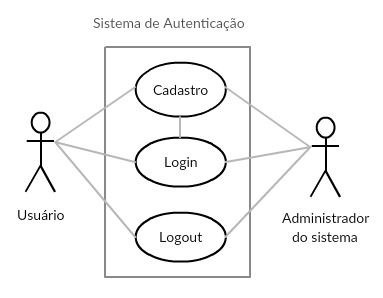
\includegraphics[scale=0.8]{img/casosautenticacao.png}
	\caption{Diagrama de Casos de Uso do Sistema de Autenticação.}
\end{figure}
\begin{figure}[!h]
	\centering
	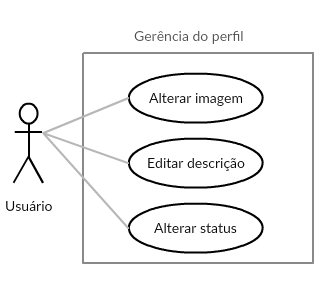
\includegraphics[scale=0.8]{img/casosperfil.png}
	\caption{Diagrama de Casos de Uso da Gerência de Perfil.}
\end{figure}
\begin{figure}[!h]
	\centering
	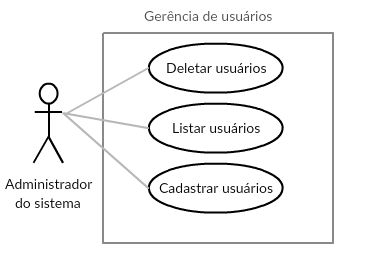
\includegraphics[scale=0.8]{img/casosusuarios.png}
	\caption{Diagrama de Casos de Uso da Gerência de Usuários.}
\end{figure}
\begin{figure}[!h]
	\centering
	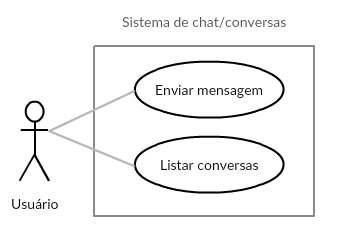
\includegraphics[scale=0.8]{img/casoschat.png}
	\caption{Diagrama de Casos de Uso do Sistema de Chat/Conversas.}
\end{figure}
\begin{figure}[!h]
	\centering
	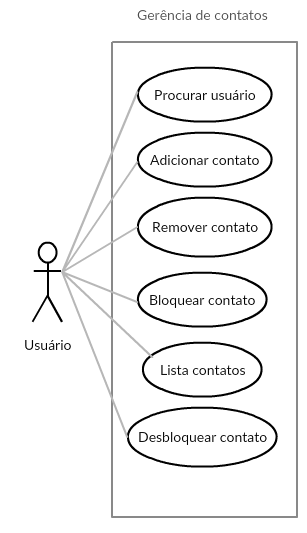
\includegraphics[scale=0.8]{img/casoscontatos.png}
	\caption{Diagrama de Casos de Uso da Gerência de Contatos.}
\end{figure}
\begin{figure}[!h]
	\centering
	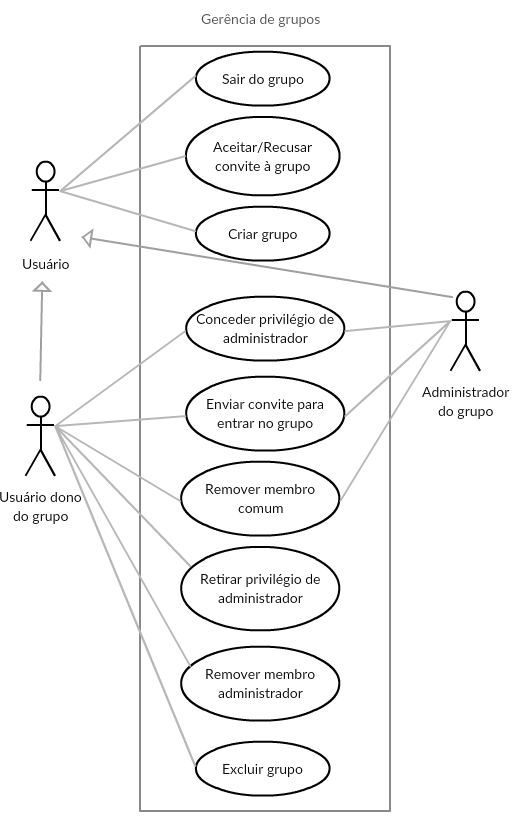
\includegraphics[scale=0.8]{img/casosgrupos.png}
	\caption{Diagrama de Casos de Uso da Gerência de Grupos.}
\end{figure}
\end{document}